\chapter{Canonical generation}
\label{ch:canonical}

Algorithm \ref{alg:one-stage} generates many permutations of the same set. This becomes a problem especially when computing $k$-bonds for $k \geq 2$ because the algorithm is then called for each of the different permutations and generates the same $k$-bond more than once.

To reduce multiple generation of $k$-bonds we implement a technique of \textit{canonical generation}. McKay in \cite{mckay_isom} both presents an overview of various approaches to canonical generation and describes in detail the technique of \textit{generation by canonical construction path} which is the basis for our approach. We start by outlining the general idea.

\subsection*{Generation by canonical construction path}

Say we are generating some \textit{labeled} objects $\vec X$ and there is an equivalence relation $\simeq$ on the set of these objects. We apply generation by canonical construction path to generate only one object from each equivalence class of $\simeq$.

For each equivalence class $\mathcal{C}$ of $\simeq$ we (carefully) choose in advance a unique \textit{canonical representative}. We denote the canonical representative $\mcan(\vec X)$ for some $\vec X \in \mathcal{C}$.

At each iteration of the generating procedure we start with a partial solution $\vec Y$ and we \textit{check} whether this augmentation of $\vec Y$ is a prefix of $\mcan(\vec X)$, where $\vec X$ is some complete solution made from $\vec Y$. Note that this check is allowed to have false positives (that is allow augmentation which does not lead to the canonical solution) but no false negatives.

At the end of the generating procedure there is a complete solution \linebreak ${\vec X = \mcan(\vec{X}) }$ and the algorithm outputs it.

\sectionline

The definition of $\mcan()$ has to be compatible with the original generating routine so it is feasible to test $X$ against this definition often in the algorithm and so it does not miss any solution. On the other hand one wants to choose $\mcan()$ such that it prunes the search tree of the generating procedure\footnote{A tree where the root marks the start of the algortihm, inner nodes contain partial solutions and leafs mark the end of a branch of computation} to the utmost possible measure.

\clearpage

\section{Canonical generation of $k$-bonds}

We apply the idea of generation by canonical construction path to Algorithm \ref{alg:one-stage}. Before continuing we suggest to recall the Definition \ref{defn:stepwise_partition}.

Let $G$ be a connected graph and $X \subseteq E(G)$ a $k$-bond. For each \break $j \in \{1, \ldots, k\}$, denote by $Z^j$ the set $\{c_{s(j)+1}, c_{s(j)+2}, \ldots, c_{s(j+1)}\}$, denote by $G^j$ the set $G \setminus \{c_{1}, \ldots, c_{s(j)}\}$ and by $G^j_0$ the connected component of $G^j$ such that $Z^j \subseteq E(G^j_0)$.

\begin{defn}[Canonical form of a stepwise partition]
	\label{can}

	Let $G$ be a connected graph, $X \subseteq E(G)$ a $k$-bond with $\lvert X \rvert = l$, $\mathcal{Z}$ a stepwise partition of $X$ and $s$ a mapping dependent on $X$ (confer Definition \ref{defn:stepwise_scheme}). Furthermore let
	$\iota : E(G) \rightarrow \{1,\ldots,\lvert E(G) \rvert\}, \> \nu : V(G) \rightarrow \{1,\ldots,\lvert V(G) \rvert\}$ be arbitrary bijections (indexing the edges and vertices) and let $\lambda : E(G) \rightarrow \mathbb{N}$ be an arbitrary mapping. The~\textit{canonical form} of $\mathcal{Z}$, $can(\mathcal{Z}) = (c_1, c_2,\ldots, c_l)$, is a permutation of $X$ which satisfies the following, for each $j \in \{1,\ldots,k-1\}$:

	\begin{enumerate}[label=\alph*.]
		\item Let $u,v$ be the ends of $c_{s(j)+1} \in Z^j$. The vertices of edges in $Z_j$ can be bipartitioned as $V(Z^j) = V^j_r \dot\bigcup V^j_b$, such that each edge of $Z^j$ has one of its ends in $V_b^j$ and the other in $V_r^j$. Moreover $u \in V_r^j$ if and only if $\nu(u) < \nu(v)$.

		\item The edge $c_{s(j)+1}$ satisfies ${\iota(c_{s(j)+1}) = \min\{ \iota(c_i) : s(j) < i \leq s(k) \}}$

	\item For each $i \in \{s(j) + 2,\ldots, s(j+1)\}$,
		let $P_{u,v} \subseteq G^j_0$ be a certain path with ends $u,v$,
		let $c_i$ be the edge of $E(P) \cap Z^j$ closest to the end $u$ in $P$ and let
		$Y_{ji} = \{c_{s(j)+1}, \ldots, c_i\} \subseteq Z^j$.

		Define $P_{u,v} \subseteq G_0^j \setminus Y_{ji}$ to be the \textit{unique shortest path}, such that among all $V_r(Y){-}V_b(Y)$ paths in $G^j_0 \setminus Y_{ji}$, it lexicographically minimizes the triplet
	$(\lvert E(P) \rvert, \mlen_\lambda(P), \vec{\iota}(P) )$, where $\mlen_\lambda(P) = \sum_{e \in E(P)} \lambda(e)$ and $\vec{\iota}(P) = (\iota(e_1), \iota(e_2),\ldots, \iota(e_{\lvert E(P) \rvert}))$.

	\end{enumerate}

\end{defn}


\noindent
\begin{note}
The first point of the above definition uses Lemma \ref{stepwise_2bond}.
\end{note}

\clearpage %%%%%%%%%%%%

\noindent
To shorten our notation we introduce $\mu$ and $\tau$ as follows.

\begin{defn}
	Let $\iota$ be an arbitrary bijection (confer Definition \ref{can}), $Z$ be a $k$-bond with stepwise partition $(Z^1,\ldots,Z^{k-1})$, $s$ be a mapping as in Definition \ref{defn:stepwise_scheme} and $1 \leq j \leq k - 1$.

\[
	\mu(Z^j) \stackrel{\text{def}}{=} \min\{ \iota(c) : \in Z^j \}
\]

\medskip

\noindent
Let $Y$ be a prefix of $Z$ and $h$ the largest index such that $c_{s(h)+1}$ belongs to $Y$.
	\[
		\tau(Y) \stackrel{\text{def}}{=}
		\begin{cases}
			\hfill -\infty    		 \hfill & \text{if $Y = \varnothing$} \\
			\hfill c_{s(h)+1} \hfill & \text{otherwise} \\
		\end{cases}
	\]
\end{defn}

\begin{defn}[Canonical form of a bond]
	\label{defn:can_bond}

	Let $G$ be a graph and $X \subseteq E(G)$ be a $k$-bond. Define $can(X)$ to be the canonical form of some stepwise partition $(Z^1,\ldots,Z^{k-1})$ of $X$, such that $\mu(Z^1) < \mu(Z^2) < \ldots < \mu(Z^{k-1})$.
\end{defn}


\begin{lem}
	\label{lem:every_kbond_has_can}
	For every $k$-bond $X$ there exists a canonical form $\vec{X}$ of $X$.
\end{lem}

\begin{proof}
	We proceed by induction on the number of stages. First we show that the edge $c_1 = c_{s(1)+1} \in \vec{X}$ satisfying (by Definition \ref{can}) $\iota(c_{s(1)+1}) = min\{ \iota(c_i) : s(1) < i \leq s(k) \}$, lies in the $\iota$-minimum $k$-way basis, that is the $\iota$-minimum spanning forest $F \subseteq G$ consisting of $k-1$ trees.

	For a contradiction suppose that $c_{s(1)+1}$ does not lie in $F$. Because $\vec X$ is a cocircuit of $G$, it intersects every basis of $G$ including the $\iota$-minimal one $F$, by Proposition \ref{matroid_folklore}. Say there is an element $e$ in the intersection of $\vec X$ with $F$. Then $F \cup \{c_{s(1)+1}\}$ contains a circuit through $e$. The set $F' = F \cup \{c_{s(1)+1}\} \setminus \{e\}$ is a basis such that

\[
	\sum_{e \in F'} \iota(e) < \sum_{e \in F} \iota(e)
\]

This contradicts the assumption that $F$ is a minimum basis.

	By Claim \ref{claim:circuit_types} and Lemma \ref{lem:stepwise_is_welldefined} the rest of the edges of this first stage can be selected as a type-C circuit. For each edge the algorithm selects the unique path (satisfying Definition \ref{can}) which is contained in an implicit type-C circuit (confer Corollary \ref{cor_circuit_subset}). This finishes the first stage.

	For the induction step consider the $j$-th stage and a $j$-bond $Y \subseteq \vec X$. We want to show that the edge $c_{s(j)+1} \in \vec X$ lies in the $\iota$-minimum type-F circuit, that is a $\iota$-minimum spanning forest $F$ on $k-2$ trees. Since $\lvert F \cap Y \rvert = 1$, it suffices to show that the edge $c_{s(j)+1}$ lies on a $\iota$-minimum spanning forest $S = F \sm Y$ on $k-1$ trees (again a $k$-way basis) such that and $Y \cap S = \varnothing$. To prove this we provide a very similar argument as in the base case:

	For a contradiction suppose that $c_{s(j)+1}$ does not lie in $S$. Because $\vec X$ is a cocircuit of $G$, it intersects every basis of $G$. Say there is an element $e$ in the intersection of $\vec X$ with $S$. Then $S \cup \{c_{s(1)+1}\}$ contains a circuit through $e$. The set $S' = S \cup \{c_{s(j)+1}\} \setminus \{e\}$ is a basis contradicting our assumption that $S$ is minimum.


	The rest of the edges of this $j$-th stage is chosen in the same way as in the first stage. This finishes the induction step.
\end{proof}

\begin{exmp*}
	The canonical form of $X$ is not unique.
	Let $k = 3$, $m = 3$. In stage 1 the algorithm generates bonds $(0,1)$ and $(0,2)$. In stage 2 bond $(0,1)$ is extended to $(0,1,2)$ and bond $(0,2)$ is extended to $(0,2,1)$.

	\begin{center}
		% 
% dot2tex --autosize tmp/graph9.tmp --prog neato --figonly
%

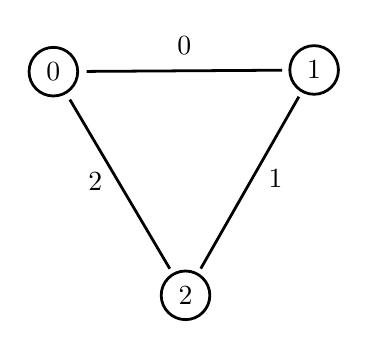
\begin{tikzpicture}[>=latex,line join=bevel,real/.append style={circle, draw=black} ]
  \pgfsetlinewidth{1bp}
%%
\pgfsetcolor{black}
  % Edge: 0 -- 1
  \draw [] (-35.2bp,26.724bp) .. controls (-15.446bp,26.841bp) and (15.392bp,27.043bp)  .. (35.2bp,27.159bp);
  \definecolor{strokecol}{rgb}{0.0,0.0,0.0};
  \pgfsetstrokecolor{strokecol}
  \draw (0bp,35.941bp) node {0};
  % Edge: 2 -- 0
  \draw [] (-5.2199bp,-44.329bp) .. controls (-14.277bp,-29bp) and (-31.973bp,0.95243bp)  .. (-41.211bp,16.588bp);
  \draw (-32.1bp,-12.8705bp) node {2};
  % Edge: 1 -- 2
  \draw [] (41.229bp,17.623bp) .. controls (32.319bp,2.0092bp) and (14.815bp,-28.662bp)  .. (5.9095bp,-44.269bp);
  \draw (32.8bp,-12bp) node {1};
  % Node: 1
\begin{scope}
  \definecolor{strokecol}{rgb}{0.0,0.0,0.0};
  \pgfsetstrokecolor{strokecol}
  \draw (46.722bp,27.249bp) node [real] {1};
\end{scope}
  % Node: 0
\begin{scope}
  \definecolor{strokecol}{rgb}{0.0,0.0,0.0};
  \pgfsetstrokecolor{strokecol}
  \draw (-47.146bp,26.633bp) node [real] {0};
\end{scope}
  % Node: 2
\begin{scope}
  \definecolor{strokecol}{rgb}{0.0,0.0,0.0};
  \pgfsetstrokecolor{strokecol}
  \draw (0.42374bp,-53.881bp) node [real] {2};
\end{scope}
%
\end{tikzpicture}


	\end{center}

\vspace{-0.5cm}
\end{exmp*}

\subsection*{Achieving the canonical generation within Algorithm \ref{alg:one-stage}}

\begin{itemize}
	\item At the beginning of each stage the edge $c$ which is being added to $X$ has to satisfy $\iota(c) > \tau(Y)$. Note that as a result the spanning forest $F$ has to be recomputed at the beginning of each stage

	\item Within each stage, after the first edge has been chosen then all the edges $c'$ being added to $X$ have to satisfy $\iota(c') > \tau(Y)$

	\item The path $P$ is chosen on line 18 such that it satisfies the condition of Definition \ref{can}.c.

	\item The choice of edge $c \in E(P) \cap Z^j$, such that it is the edge in $E(P) \cap Z^j$ closest to $T_r$, is embedded in the algorithm by iterating through the edges of $P$ \textit{in order} ("red $\rightarrow$ blue")

\end{itemize}

\clearpage

\begin{algorithm}
	\caption{One canonical stage of stepwise implementation}
	\label{alg:can_one_step}
\begin{algorithmic}[1]
	\Require A connected graph $G$, parameters $j,\, k,\, m \in \mathbb{N},\, j < k,\, m \geq 1$ and a~$j$-bond $Y_1 \subseteq E(G)$
	\Ensure A collection of $(j+1)$-bonds as in Algorithm \ref{alg:one-stage}), such that each one is in the unique canonical form extending $Y_1$

	\If{$j=1$}
		\State $F \leftarrow$ a $\iota$-minimum spanning forest of $k-1$ trees
		\Else
		\State $F \leftarrow$ a $\iota$-minimum spanning forest of $k-2$ trees, $\lvert F \cap Y_1 \rvert = 1$
	\EndIf

	\ForAll{$d = \{u, v\} \in F \setminus \{e \in E(G) \mid \iota(e) \leq \tau(Y_1) \} $}
		\State \textbf{if} $ \, \nu(v) < \nu(u)$ \textbf{then}  $u,v \leftarrow v, u \,$ \textbf{fi}
		\State \Call{GenStage}{$j, Y_1, X = \{d\}, V_r = \{u\}, V_b = \{v\}, T_r = \{u\}$}
	\EndFor

	\Procedure{GenStage}{$j, Y, X, V_r, V_b, T_r$}
	\State Let $G_1 \subseteq G$ be the conn. component of $G \setminus Y$ containing $X$
	\If{$\lvert Y \cup X \rvert > m - k + j + 1$}
		\State \textbf{return $\undefined$}
	\EndIf
	\If{there does not exist a connected subgraph \\ \qquad \enspace  $T_b \subseteq (G_1 \setminus V(T_r)) \setminus X$ such that $V_b \subseteq V(T_b)$}
		\State \textbf{return $\undefined$}
	\EndIf
	\State $P' \leftarrow$ a path $P' \subseteq G_1$ connecting some $r \in V_r$ and $b \in V_b$ \\
	\qquad \quad \,\,\, minimizing $(\lvert E(P) \rvert, \mlen_\lambda(P), \vec{\iota}(P) )$
	\State $P \leftarrow P' \setminus T_r$
	\If{such $P$ does not exist}
		\State \textbf{return} $Y \cup X$ \Comment{$Y \cup X$ is a $j+1$-bond}
	\Else
		\ForAll{$c \in P$}
			\If{$\iota(c) < \tau(Y \cup X)$}
				\State \textbf{continue}
			\EndIf
			\State Let $u$ be the vertex in $c = \{u,v\}$ which is closer to $T_r$
			\State Let $P_u$ be the component of $P - c$ which contains $u$
			\State \Call{GenStage}{$j, Y, X \cup \{c\}, V_r \cup \{u\}, V_b \cup \{v\}, T_r \cup P_u$}
		\EndFor
	\EndIf

	\EndProcedure
\end{algorithmic}
\end{algorithm}

\clearpage


\begin{lem}
	\label{lem:alg_is_canonical}
	Let $G$ be a connected graph. If an implementation of Algorithm \ref{alg:one-stage} satisfies the conditions of Definition \ref{can}, namely

	\begin{itemize}
		\item the spanning forest selected at the beginning of each stage (in \textsc{ExtendBond}) is chosen such that it is the unique minimal one with respect to edge weights $\iota$
		\item each path $P$ is chosen such that it lexicographically minimizes the triplet $(\lvert E(P) \rvert, \mlen_\lambda(P), \vec{\iota}(P) )$
	\end{itemize}

	then every generated partition $\mathcal{Z}$ of each $k$-bond $X \subseteq E(G)$ is in its canonical form $can(\mathcal{Z})$.
\end{lem}

\begin{proof}
	Directly from Algorithm \ref{alg:can_one_step}.
	\begin{itemize}
		\item The condition \ref{can}.a is satisfied due to line 7.
		\item The condition \ref{can}.b is satisfied by choosing the minimum spanning forest on lines 2, 4 and by the condition on line 26.
		\item The condition \ref{can}.c is satisfied by the choice of $P$ on line 19.
	\end{itemize}
\end{proof}

\noindent The following theorem is a direct consequence of Theorem \ref{thm:stepwise_impl_correctness} and Lemma \ref{lem:every_kbond_has_can}.


% TODO: Is the "\vec X = \mcan(X)" part allowed with the current definition of can(X), where X is a bond?
\begin{thm}
	Let $G$ be a graph, $k \geq 2$, $m \geq 1$ integers. Recursive application of Algorithm \ref{alg:can_one_step} generates at least one canonical form $\vec X = \mcan(X)$ of every $k$-bond $X \subseteq E(G)$, $\lvert X \rvert \leq m$.
\end{thm}

The corollary below allows the implementation to slightly differ from the definition of $\mcan()$ without losing correctness. This changes our further use of the term \textit{unique shortest path}.

\begin{cor}
	Algorithm \ref{alg:can_one_step} can be modified to always choose the unique shortest path to be a $V(T_r){-}V_b$ path.
\end{cor}

This unique shortest path can omit the edges of $T_r$ since they were already in $X$ in a different branch of computation.

\begin{claim}
	\label{forest_sel_claim}
	Algorithm \ref{alg:can_one_step} remains correct if in the first step, for both $j = 1$ and $j \leq 2$, it selects $F$ as the minimum spanning forest ${F \subseteq (G \setminus Y)}$ consisting of $k-1$ trees.
\end{claim}

\section{Complete algorithm}

In this section we provide the final version of the circuit-cocircuit algorithm which is used for our practical implementation. Before doing so we introduce several small changes.


\subsection*{Heuristic for the test of hyperplane existence}
Recall that in a given graph $G$ we are avoiding non-minimal cuts $X \subseteq E(G)$ by using a test for the existence of a hyperplane of $G$ in $G \setminus X$. As a helper tool we are using colouring of the graph as described previously.

Previously, we used a basic hyperplane existence test based on performing a graph traversal each time an edge is added to $X$. Now we propose a heuristic which avoids repeated traversal.

\begin{claim}
	Let $G$ be a graph and $X \subseteq E(G)$. Assume there is a blue subgraph interconnecting $V_b$ and perform \textit{check} for a possible disconnection each time some edge $c$ is added to $X$. If this check is positive then a graph traversal is performed and, if possible, a new subgraph interconnecting $V_b$ is found. This \textit{check} can be a heuristic with false positives but no false negatives.
\end{claim}

To implement this technique, the algorithm has a variable for a connected blue subgraph $G_b \subseteq (G \setminus T_r) \setminus X$ such that $V_b \subseteq G_b$. When adding some edge $c$ to $X$ we \textit{check} whether this causes disconnection of $G_b$ with a method which treats $G_b$ as a tree, resulting in a quick test. In case this \textit{check} is positive we attempt to find ("re-create") a new connected subgraph $G_b' \subseteq (G \setminus T_r) \setminus X$ such that $V_b \subseteq V(G_b')$. If $G_b'$ could not be found the algorithm skips further computations using $X \cup \{c\}$. If $G_b'$ was found the algorithm continues its operation with $X \cup \{c\}$ and $G_b := G_b'$.

As suggested the assumption that $G_b$ is a tree may not be correct\footnote{This may happen due to the choice of paths in the "re-creation" procedure and in the \lstinline|shortestPath| procedure} -- in this case the test reported false positive and a new connected blue subgraph $G_b' \subseteq G$ such that $V_b \subseteq V(G_b)$ is found although the previous one might have been connected.

Details on implementing \textit{check} and finding a new ("re-creating") blue subgraph are given in Chapter \ref{ch:practical_impl}.

\subsection*{Aborting \lstinline|GenStage| after losing a hyperplane}

\begin{claim}
	Algorithm \ref{alg:can_one_step} may end the execution of a \lstinline|GenStage| call right after adding $c$ to $X$ if it results in $G \setminus X$ having no hyperplane of $G$.
\end{claim}

\sectionline

Algorithm \ref{alg:final} shows the recursive composition of Algorithm \ref{alg:can_one_step} with above mentioned minor improvements. This is the final version of our algorithm and will serve as a~basis for the practical implementation.

\clearpage

\begin{algorithm}
	\caption{Canonical stepwise Circuit-Cocircuit algorithm}
	\label{alg:final}
\begin{algorithmic}[1]
	\Require A connected graph $G$, parameters $k,m \in \mathbb{N}, m \geq 1$
	\Ensure All $k$-way bonds of $G$ in a canonical form and with $\leq m$ edges

	\State \Call{ExtendBond}{$j = 1, Y = \varnothing, V_r = \varnothing, V_b = \varnothing, T_r = \varnothing, G_b = \varnothing$}
	\Procedure{ExtendBond}{$j, Y, V_r, V_b, T_r, G_b$}
	\State $F \leftarrow$ $\iota$-minimum spanning forest $F \subseteq (G \setminus Y )$ on $k-1$ trees
	\ForAll{$d = \{u, v\} \in F \setminus \{e \in E(G) \mid \iota(e) < \tau(Y) \}$}
		\State \textbf{if} $ \, \nu(v) < \nu(u)$ \textbf{then}  $u,v \leftarrow v, u \,$ \textbf{fi}
		\State \Call{GenStage}{$j, Y, \{d\}, \{u\}, \{v\}, \{u\}, \{v\}$}
	\EndFor
	\EndProcedure

	\Procedure{GenStage}{$j, Y, X, V_r, V_b, T_r, G_b$}

	\State Let $G_1 \subseteq G$ be the conn. component of $G \setminus Y$ containing $X$

	\If{$\lvert Y \cup X \rvert > m - k + j + 1$}
		\State \textbf{return $\undefined$}
	\EndIf

	\State $P \leftarrow$ a path $P \subseteq G_1$ connecting some $r \in V(T_r)$ and $b \in V_b$ \\
	\qquad \quad \,\,\, minimizing $(\lvert E(P) \rvert, \mlen_\lambda(P), \vec{\iota}(P) )$

	\If{such $P$ does not exist}
		\State \textbf{if} $j = k - 1$ \textbf{then} \textbf{return} $Y \cup X$ \Comment{$X$ is a $k$-bond}
		\State \textbf{else} \Call{ExtendBond}{$j + 1, Y \cup X, \varnothing, \varnothing, \varnothing, \varnothing$} \textbf{fi}

	\Else
		\ForAll{$c = \{u, v\} \in P$}
			\State Let $u$ be the vertex in $\{u,v\}$ which is closer to $T_r$
			\State Let $P_u$ be the component of $P - c$ which contains $u$
			\State Let $P_v$ be the component of $P - c$ which contains $v$
			\If{$G_b \sm \{c\}$ is disconnected}
				\State $G_b \leftarrow$ a new subgraph interconnecting $V_b$
				\State \textbf{if} such $G_b$ cannot be found \textbf{then} \textbf{return $\undefined$}
			\EndIf
			\If{$\iota(c) < \tau(Y \cup X)$}
				\State \textbf{continue}
			\EndIf
			\State \textsc{GenStage}($j, Y, X \cup \{c\}, V_r \cup \{u\}, V_b \cup \{v\},$ \\
			\hskip 116.8pt $T_r \cup P_u, G_b \cup P_v$)
		\EndFor
	\EndIf

	\EndProcedure
\end{algorithmic}
\end{algorithm}

